\chapter{Results} \label{ch4:resu}

This chapter contains the results, using the implementations explained in the previous chapter. All of the experiments were performed on a computer with an i7-4900MQ Processor (2.8 GHz Quadcore). Note however that the code was not optimized to take advantage of the multiple cores, to make use of multithreading, or to use GPU hardware acceleration.

As there are, given an environment with $l$ links and $o$ obstacles, two ways of running the \gls{SQ} collision detection method, both are used in the testing. In the following these are called O\gls{SQ} and R\gls{SQ}, which stand for Obverse-\gls{SQ} and Reverse-\gls{SQ} respectively. In O\gls{SQ} the links are represented implicitly and the obstacles explicitly, whereas in R\gls{SQ} obstacles are represented implicitly and the links explicitly.

\section{Comparing Collision Detection Methods}

In this section, the three collision detection methods are compared with each other in four rounds of tests. Each test round aims to challenge the algorithms in a distinct way.

\subsection{Collision Detection: True Negatives} \label{subsec:Test1}

In the first round of tests, the aim was to see how fast the algorithms terminate when there are no collisions. The obstacle shapes were spherical ($a_1=a_2=a_3=5$, $\epsilon_1=\epsilon_2 = 1)$ and the links ($a_1=a_2=1$, $a_3=10$, $\epsilon_1=0.7$, $\epsilon_2 = 1$) prolate spheroids. Note that the links were all placed on a box-shaped \gls{SQ} base, which added to the number of links and, the \gls{DoF}, by one. Table \ref{Table:1} contains the results of this test round.
\begin{table}[h]
	\centering
	\caption{Table showing the results of the first round of tests. The bold and underlined values are the quickest times.}
	\begin{tabular}{|l|c|c|c|c|c|c|}
		\hline
Test: & $n^2$ & $l$	& $o$ & \gls{GJK} [s] & O\gls{SQ} [s] & R\gls{SQ} [s]\\
\hline
		1.I 	& $80^2$	&	2	&	1	&	0.1420000	&	0.1599998   &	\underline{\textbf{0.1399999}}	\\
		1.II 	& $80^2$	&	2	&	4	&	0.5679998	&	0.6619999   &	\underline{\textbf{0.5500000}}	\\
		1.III	& $80^2$  &	2	&	6	&	\underline{\textbf{0.7830000}}	&	0.9519999   &	0.9399998	\\
		1.IV	& $80^2$  &	2	&	12	&	1.3030000	&	1.4630001   &	\underline{\textbf{1.2670000}}	\\
		1.V		& $80^2$	&	4	&	1	&	0.5859999	&	0.5869999   &	\underline{\textbf{0.5300000}}	\\
		1.VI	& $80^2$	&	4	&	4	&	\underline{\textbf{1.1200001}}	&	1.1340000	&	1.5039999	\\
		1.VII	& $80^2$	&	4	&	6	&	\underline{\textbf{1.6449999}}	&	2.0280001	&	1.8030000	\\
		1.X		& $80^2$	&	4	&	12	&	2.6849999	&	2.955000	&	\underline{\textbf{2.648000}}	\\		
		1.IX	& $80^2$	&	6	&	1	&	0.8770001	&	0.8309999	&	\underline{\textbf{0.8090000}}	\\
		1.X		& $80^2$	&	6	&   4	&	\underline{\textbf{1.8080001}}	&	1.8940001	&	1.8220000	\\
		1.XI 	& $80^2$	&	6	&   6	&	\underline{\textbf{2.6629999}}	&	2.5239999	&	2.9459999	\\
		1.XI 	& $80^2$	&	6	&   12	&	3.9990001	&	4.3389999	&	\underline{\textbf{3.9619999}}	\\
		\hline         
	\end{tabular}
	\label{Table:1}
\end{table}

\begin{figure}[h]
	\centering
	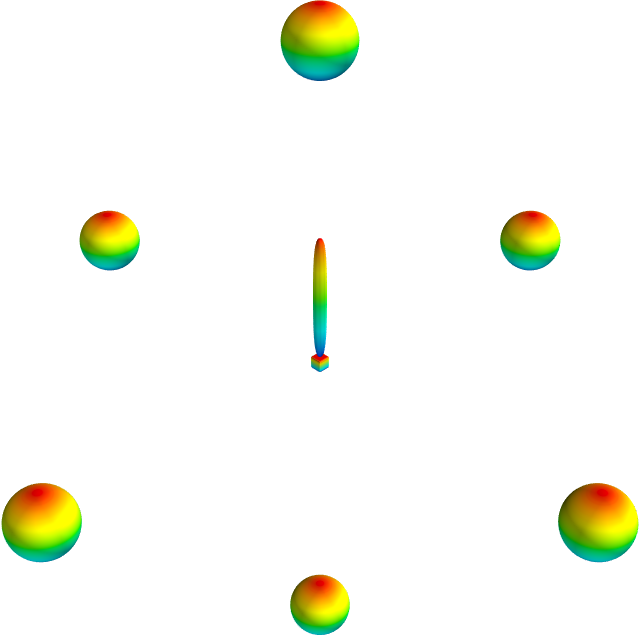
\includegraphics[width=0.35\textwidth]{/import/Test1_III}
	\caption{Visualization of Test 1.III.}
	\label{fig:Test1III}
\end{figure}

$i_{max}$ is presented here though it had no bearing on the terminations of the \gls{GJK} algorithm instances; they all terminated in accordance with Termination Condition 1. Figure \ref{fig:Test1III} visualizes Test 1.III (two links, six obstacles). Obstacles have been placed in pairs along the $x$, $y$ and $z$ axes around the arm, which was kept in that upright position. For the later tests with more links, the top spherical obstacle was translated sideways in order to avoid collision.

\subsection{Collision Detection: True Positives}\label{subsec:Test2}

In the second round of tests, the algorithms were tested on how fast they detect a collision. Using  6 \gls{DoF} arm (assuming that all the joints are revolute joints), various constellations of collision scenarios were tested. The links and obstacle were the same shapes as the test round in Section \ref{subsec:Test1}. One obstacle was used, which intersected with each of the links individually. Table \ref{Table:2} contains the result of this test round.

\begin{table}[h]
	\centering
	\caption{Table showing the results of the second round of tests. The bold and underlined values are the quickest times.}
	\begin{tabular}{|l|c|c|c|c|c|c|}
		\hline
		Test: & $n^2$ & Collision & $i_{max}$ & \gls{GJK} [s] & O\gls{SQ} [s] & R\gls{SQ} [s]\\
		\hline
		2.I 	& $80^2$	&	Link 0	&	50	&	0.1139998	&	0.3239999   &	\underline{\textbf{0.0007000}}	\\
		2.II 	& $80^2$	&	Link 1	&	50	&	0.3740001	&	0.3050001   &	\underline{\textbf{0.0719998}}	\\
		2.III 	& $80^2$	&	Link 2	&	50	&	0.4330001	&	0.2920001   &	\underline{\textbf{0.1240001}}	\\
		2.IV 	& $80^2$	&	Link 3	&	50	&	0.3170002	&	0.4480000   &	\underline{\textbf{0.1790001}}	\\
		2.V 	& $80^2$	&	Link 4	&	50	&	0.5440002	&	0.3099999	&	\underline{\textbf{0.2300000}}	\\
		2.VI 	& $80^2$	&	Link 5	&	50	&	0.6230001	&	\underline{\textbf{0.2909999}}	&	0.3079999	\\
		\hline         
	\end{tabular}
	\label{Table:2}
\end{table}

The \gls{GJK} algorithm had an average time of $0.4008334$ seconds, compared to the $0.3283333$ seconds and the $0.1522833$ seconds average times of the O\gls{SQ} and R\gls{SQ} algorithms respectively. 

Figure \ref{fig:Test2VI} illustrates how the obstacle was moved along the $z$-axis. The \gls{GJK} algorithm all terminated due to the algorithm being able to encapsulate the origin in a $4$-simplex, i.e. Termination Condition 3.
\begin{figure}[h]
	\centering
	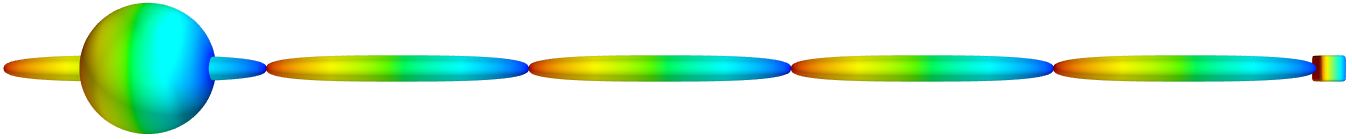
\includegraphics[width=0.8\textwidth]{/import/Test2_VI}
	\caption{Visualization of Test 2.VI. The $z$-axis is horizontally positive to the left.}
	\label{fig:Test2VI}
\end{figure}
It was however discovered while testing that if the obstacle is translated by 25 units in the positive $z$-axis, as shown in Figure \ref{fig:Test2max}, the \gls{GJK} algorithm will have problems and terminate in accordance with Termination Condition 4. As the maximum iteration limit $i_{max}$ is set to 50, this resulted in a computation time of 1.275000 seconds.
\begin{figure}[h]
	\centering
	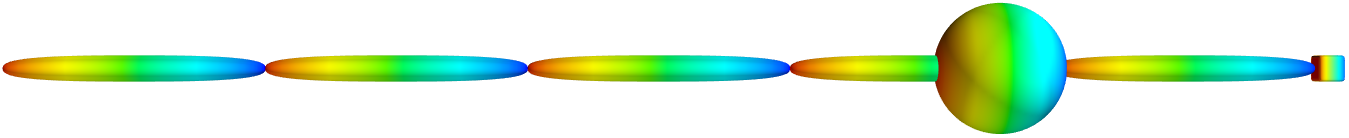
\includegraphics[width=0.8\textwidth]{/import/Test2_maxIter}
	\caption{Visualization of a particularly troublesome case for the GJK algorithm. The obstacle has been translated 25 units along the positive $z$-axis.}
	\label{fig:Test2max}
\end{figure}

\subsection{Varying Number of Object Points}\label{subsec:Test3}

In the previous test rounds of Sections \ref{subsec:Test1} and \ref{subsec:Test2}, $n$ was kept at $80$. This means that the points, of total number $80^2$, were sampled with increments of $\frac{pi}{80}$ radians (2.25 degrees) and $\frac{pi}{40}$ radians (4.5 degrees) for $\eta$ and $\omega$ respectively. The aim of this test round was to see how the algorithms fare when the total number of points change. Or, in other words, when the point density changes. 

In all the tests, there was one spherical obstacle as well as an arm with the base (link 0) and one more link. They did not intersect. The results are shown in Table \ref{Table:3}.

\begin{table}[h]
	\centering
	\caption{Table showing the results of the third round of tests. The bold and underlined values are the quickest times.}
	\begin{tabular}{|l|c|c|c|c|}
		\hline
		Test: 	& $n^2$ &   \gls{GJK} [s] & O\gls{SQ} [s] & R\gls{SQ} [s]\\
		\hline
		3.I 	&	$10^2$		&	0.0060000	&	\underline{\textbf{0.0030000}}	&	0.0040000	\\
		3.II 	&	$20^2$		&	0.0190001	&	0.0100000	&	\underline{\textbf{0.0079999}}	\\
		3.III 	&	$50^2$		&	0.0639999	&	0.0520000	&	\underline{\textbf{0.0480001}}	\\
		3.IV 	&	$80^2$		&	0.1580000	&	0.1170001	&	\underline{\textbf{0.1069999}}	\\
		3.V 	&	$100^2$		&	\underline{\textbf{0.2010000}}	&	0.2180002	&	0.2230000	\\
		3.VI 	&	$150^2$		&	0.4600000	&	0.5349998	&	\underline{\textbf{0.4470000}}	\\
		3.VII 	&	$200^2$		&	0.9840000	&	0.8140001	&	\underline{\textbf{0.7579999}}	\\
		3.VIII 	&	$300^2$		&	1.9730000	&	1.7790000	&	\underline{\textbf{1.7070000}}	\\
		3.IX	&	$500^2$		&	\underline{\textbf{4.5090000}}	&	4.8710001	&	4.6440001	\\
		3.X		&	$1000^2$	&	\underline{\textbf{19.0970001}}	&	19.1299999	&	20.3789999	\\
		\hline         
	\end{tabular}
	\label{Table:3}
\end{table}

\subsection{Large Number of Objects} \label{subsec:Test4}
The purpose of this test round was to examine how the algorithms were affected by truly large number of objects, both in terms of many links and in terms of many obstacles. $n^2 = 6400$ for all the values listed in Table \ref{Table:4}.

\begin{table}[h]
	\centering
	\caption{Table showing the results of the fourth round of tests. The bold values are the quickest times.}
	\begin{tabular}{|l|c|c|c|c|c|}
		\hline
		Test: 	&	$l$		&	$o$	&	\gls{GJK} [s] & O\gls{SQ} [s] & R\gls{SQ} [s]\\
		\hline
		4.I 	&	1001	&	1	&	\underline{\textbf{58.779000}}	&	64.878999	&	62.555999	\\
		4.II 	&	2501	&	1	&	159.03400	&	165.02100	&	\underline{\textbf{158.38899}}	\\
		4.III 	&	5001	&	1	&	352.58500	&	339.92200	&	\underline{\textbf{309.05500}}	\\
\hline
		4.IV 	&	2		&	500	&	56.187000	&	57.055000	&	\underline{\textbf{55.895000}}	\\
		4.V 	&	2		&	1000&	\underline{\textbf{124.67700}}	&	131.08800	&	125.52399	\\
		4.VI 	&	2		&	2500&	296.88299	&	293.21700	&	\underline{\textbf{291.88700}}	\\
		\hline         
	\end{tabular}
	\label{Table:4}
\end{table}


\section{RRT 6 Degrees of Freedom} \label{subsec:TestRRT}

The collision detection algorithms have been implemented as black box methods that can be used interchangeably within the \gls{RRT} algorithm. A robotic arm with 6 \gls{DoF} is used, with one obstacle preventing the arm from reaching the goal configuration.

The arm links are considered to be revolute joints that can rotate around the $y$-axis ($\theta$ Euler angle) only. Thus, in this case, the arm moves in the $x$-$z$-plane. The base (link 0) is fixed, such that a five link arm represents 4 \gls{DoF}. $n^2=20^2$, the obstacle shape was spherical ($a_1=a_2=a_3=5$, $\epsilon_1=\epsilon_2 = 1)$, shifted 50 length units in the positive $x$-axis; and the links ($a_1=a_2=1$, $a_3=10$, $\epsilon_1=0.7$, $\epsilon_2 = 1$) were prolate spheroids.

Table \ref{Table:RRT_all} contains the experiment data. Six tests were done for each algorithm.
%\subsection{Three Degrees of Freedom}
%
%\begin{figure}[h]
%	\centering
%	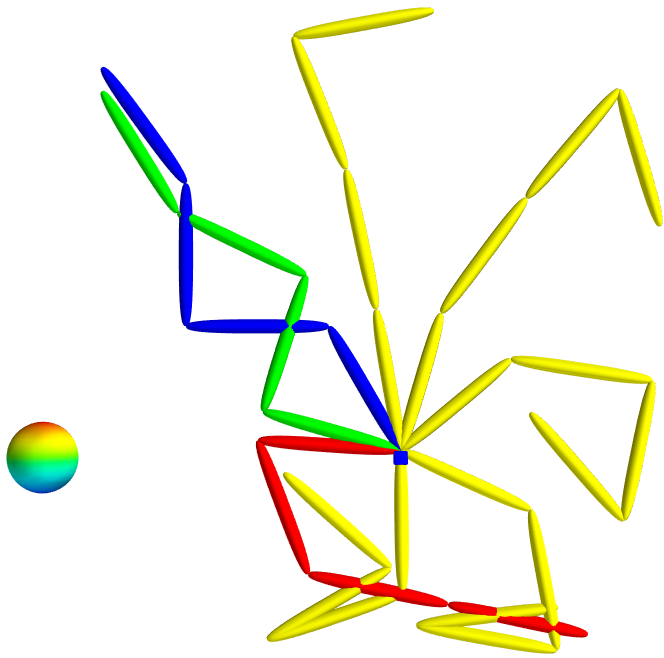
\includegraphics[width=0.8\textwidth]{/import/RRT_4DOF}
%	\caption{Arm configuration nodes produced by the \gls{RRT} algorithm. Red is the starting configuration, green is the goal configuration, blue is an accepted end configuration and the yellow are intermediary configurations.}
%	\label{fig:4DOF}
%\end{figure}
%
%Goal: [[0, 0, 0], [0, np.pi/6, 0], [0, np.pi/3, 0], [0, -np.pi/2, 0]]
%
%[[0.0, 0.0, 0.0], [0.0, -5.19025317165312, 0.0], [0.0, 0.11233734263475836, 0.0], [0.0, -7.6916774826832635, 0.0]]
%[[0.0, 0.0, 0.0], [0.0, -3.1996810478552318, 0.0], [0.0, 0.14878085122722967, 0.0], [0.0, -5.048601834477622, 0.0]]
%[[0.0, 0.0, 0.0], [0.0, -1.6429980501130528, 0.0], [0.0, 0.6138800935202502, 0.0], [0.0, -3.5591732518384975, 0.0]]
%[[0.0, 0.0, 0.0], [0.0, -1.2728589918138258, 0.0], [0.0, 0.7924096318012435, 0.0], [0.0, -2.9352796165666017, 0.0]]
%[[0.0, 0.0, 0.0], [0.0, 1.0231797436369352, 0.0], [0.0, 0.7951166673387806, 0.0], [0.0, -0.3335952867208767, 0.0]] 
%[[0, 0, 0], [0, 1.5, 0], [0, 2, 0], [0, 1, 0]] START
%
%Total loop counts: 379
%Total time 58.091000.
%
%
%\subsection{Four Degrees of Freedom}
%
%
%Goal: [[0, 0, 0], [0, np.pi/6, 0], [0, np.pi/3, 0], [0, -np.pi/2, 0], [0, np.pi/5, 0]]
%
%[[0.0, 0.0, 0.0], [0.0, -4.986947266383945, 0.0], [0.0, -1.6038593337248848, 0.0], [0.0, -4.854962684997878, 0.0], [0.0, -6.848675068496268, 0.0]]
%[[0.0, 0.0, 0.0], [0.0, -3.1288813502224153, 0.0], [0.0, -1.254834685488938, 0.0], [0.0, -2.9451331278248345, 0.0], [0.0, -4.391625670607787, 0.0]]
%[[0.0, 0.0, 0.0], [0.0, -1.997744330774695, 0.0], [0.0, -0.9594706875158981, 0.0], [0.0, -1.9305951643711614, 0.0], [0.0, -2.8379630446232116, 0.0]]
%[[0.0, 0.0, 0.0], [0.0, -0.8794533715753459, 0.0], [0.0, -0.8412105287762854, 0.0], [0.0, -1.622334778430683, 0.0], [0.0, -2.2248682493660805, 0.0]]
%[[0.0, 0.0, 0.0], [0.0, -0.2865006608526038, 0.0], [0.0, -0.3520153117927673, 0.0], [0.0, -0.06733011090080032, 0.0], [0.0, -2.146772111520897, 0.0]]
%[[0.0, 0.0, 0.0], [0.0, 0.17248987969087182, 0.0], [0.0, 0.03910929310533873, 0.0], [0.0, 0.1660034998827522, 0.0], [0.0, -1.7678726496256758, 0.0]]
%[[0, 0, 0], [0, 1.5, 0], [0, 2, 0], [0, 1, 0], [0, 0, 0]] START
%
%---
%
%[9202, 8787, 8350, 6002, 8, 7, 2, 0]
%('total count:', 10281)
%('RRT: ', 2104.8980000019073)
%[[[0.0, 0.0, 0.0], [0.0, -6.152729998813503, 0.0], [0.0, -5.469243435895454, 0.0], [0.0, -5.779452084317896, 0.0], [0.0, -7.452545072813811, 0.0]], [[0.0, 0.0, 0.0], [0.0, -4.346376070347128, 0.0], [0.0, -3.607909879552337, 0.0], [0.0, -3.9029258529393, 0.0], [0.0, -5.03383308527894, 0.0]], [[0.0, 0.0, 0.0], [0.0, -3.0023729530645644, 0.0], [0.0, -2.606479640879316, 0.0], [0.0, -2.708776059397553, 0.0], [0.0, -3.358354102941128, 0.0]], [[0.0, 0.0, 0.0], [0.0, -2.0002667322469274, 0.0], [0.0, -1.9274431597061894, 0.0], [0.0, -1.8440675408567118, 0.0], [0.0, -2.2233123518599287, 0.0]], [[0.0, 0.0, 0.0], [0.0, -1.5026324558485136, 0.0], [0.0, -1.6239947450511785, 0.0], [0.0, -1.457480642103436, 0.0], [0.0, -1.4927394978714965, 0.0]], [[0.0, 0.0, 0.0], [0.0, -1.2978780593270423, 0.0], [0.0, 0.922799407646467, 0.0], [0.0, -1.0698002300075635, 0.0], [0.0, -1.360358820056423, 0.0]], [[0.0, 0.0, 0.0], [0.0, -0.1992289553890969, 0.0], [0.0, 1.543185704028021, 0.0], [0.0, -0.7806343818040391, 0.0], [0.0, -0.683222228702385, 0.0]], [[0, 0, 0], [0, 1.5, 0], [0, 2, 0], [0, 1, 0], [0, 0, 0]]]
%[[0.0, 0.0, 0.0], [0.0, -6.152729998813503, 0.0], [0.0, -5.469243435895454, 0.0], [0.0, -5.779452084317896, 0.0], [0.0, -7.452545072813811, 0.0]]
%[[0.0, 0.0, 0.0], [0.0, -4.346376070347128, 0.0], [0.0, -3.607909879552337, 0.0], [0.0, -3.9029258529393, 0.0], [0.0, -5.03383308527894, 0.0]]
%[[0.0, 0.0, 0.0], [0.0, -3.0023729530645644, 0.0], [0.0, -2.606479640879316, 0.0], [0.0, -2.708776059397553, 0.0], [0.0, -3.358354102941128, 0.0]]
%[[0.0, 0.0, 0.0], [0.0, -2.0002667322469274, 0.0], [0.0, -1.9274431597061894, 0.0], [0.0, -1.8440675408567118, 0.0], [0.0, -2.2233123518599287, 0.0]]
%[[0.0, 0.0, 0.0], [0.0, -1.5026324558485136, 0.0], [0.0, -1.6239947450511785, 0.0], [0.0, -1.457480642103436, 0.0], [0.0, -1.4927394978714965, 0.0]]
%[[0.0, 0.0, 0.0], [0.0, -1.2978780593270423, 0.0], [0.0, 0.922799407646467, 0.0], [0.0, -1.0698002300075635, 0.0], [0.0, -1.360358820056423, 0.0]]
%[[0.0, 0.0, 0.0], [0.0, -0.1992289553890969, 0.0], [0.0, 1.543185704028021, 0.0], [0.0, -0.7806343818040391, 0.0], [0.0, -0.683222228702385, 0.0]]
%[[0, 0, 0], [0, 1.5, 0], [0, 2, 0], [0, 1, 0], [0, 0, 0]] start
%
%bias 50
%
%\subsection{Five Degrees of Freedom}
%
%[1081, 940, 798, 20, 9, 5, 2, 1, 0]
%('total count:', 1420)
%('RRT: ', 312.28799986839294)
%[[[0.0, 0.0, 0.0], [0.0, -5.711296354774484, 0.0], [0.0, -7.704167590187523, 0.0], [0.0, -4.558214116438215, 0.0], [0.0, -6.384260710917641, 0.0], [0.0, -6.28010516816726, 0.0]], [[0.0, 0.0, 0.0], [0.0, -3.4012441472811212, 0.0], [0.0, -5.003956117408275, 0.0], [0.0, -4.044193266945362, 0.0], [0.0, -4.649998042153884, 0.0], [0.0, -3.9794246609166875, 0.0]], [[0.0, 0.0, 0.0], [0.0, -1.425484503888736, 0.0], [0.0, -3.1480627825781804, 0.0], [0.0, -3.806417239200629, 0.0], [0.0, -3.389721313919457, 0.0], [0.0, -3.604439449841329, 0.0]], [[0.0, 0.0, 0.0], [0.0, -1.3167294811111412, 0.0], [0.0, -1.4281147124934774, 0.0], [0.0, -3.7247154143988115, 0.0], [0.0, -2.7713908890786842, 0.0], [0.0, -3.356672799821607, 0.0]], [[0.0, 0.0, 0.0], [0.0, -1.2891687369589924, 0.0], [0.0, 1.0695424978858887, 0.0], [0.0, -3.5779784377764687, 0.0], [0.0, -2.4206795632534535, 0.0], [0.0, -2.1724534982079384, 0.0]], [[0.0, 0.0, 0.0], [0.0, -0.8620782398324056, 0.0], [0.0, 1.9800715208841226, 0.0], [0.0, -2.4820947696095073, 0.0], [0.0, -0.7892097825846471, 0.0], [0.0, -1.9070905222437755, 0.0]], [[0.0, 0.0, 0.0], [0.0, -0.2362174973258695, 0.0], [0.0, 2.4118299370908827, 0.0], [0.0, -1.4876352840495193, 0.0], [0.0, -0.430484872232175, 0.0], [0.0, -1.7914453573637732, 0.0]], [[0.0, 0.0, 0.0], [0.0, 1.7617993877991494, 0.0], [0.0, 2.5235987755982987, 0.0], [0.0, 0.21460183660255172, 0.0], [0.0, 0.3141592653589793, 0.0], [0.0, -0.3141592653589793, 0.0]], [[0, 0, 0], [0, 1.5, 0], [0, 2, 0], [0, 1, 0], [0, 0, 0], [0, 0, 0]]]
%[[0.0, 0.0, 0.0], [0.0, -5.711296354774484, 0.0], [0.0, -7.704167590187523, 0.0], [0.0, -4.558214116438215, 0.0], [0.0, -6.384260710917641, 0.0], [0.0, -6.28010516816726, 0.0]]
%[[0.0, 0.0, 0.0], [0.0, -3.4012441472811212, 0.0], [0.0, -5.003956117408275, 0.0], [0.0, -4.044193266945362, 0.0], [0.0, -4.649998042153884, 0.0], [0.0, -3.9794246609166875, 0.0]]
%[[0.0, 0.0, 0.0], [0.0, -1.425484503888736, 0.0], [0.0, -3.1480627825781804, 0.0], [0.0, -3.806417239200629, 0.0], [0.0, -3.389721313919457, 0.0], [0.0, -3.604439449841329, 0.0]]
%[[0.0, 0.0, 0.0], [0.0, -1.3167294811111412, 0.0], [0.0, -1.4281147124934774, 0.0], [0.0, -3.7247154143988115, 0.0], [0.0, -2.7713908890786842, 0.0], [0.0, -3.356672799821607, 0.0]]
%[[0.0, 0.0, 0.0], [0.0, -1.2891687369589924, 0.0], [0.0, 1.0695424978858887, 0.0], [0.0, -3.5779784377764687, 0.0], [0.0, -2.4206795632534535, 0.0], [0.0, -2.1724534982079384, 0.0]]
%[[0.0, 0.0, 0.0], [0.0, -0.8620782398324056, 0.0], [0.0, 1.9800715208841226, 0.0], [0.0, -2.4820947696095073, 0.0], [0.0, -0.7892097825846471, 0.0], [0.0, -1.9070905222437755, 0.0]]
%[[0.0, 0.0, 0.0], [0.0, -0.2362174973258695, 0.0], [0.0, 2.4118299370908827, 0.0], [0.0, -1.4876352840495193, 0.0], [0.0, -0.430484872232175, 0.0], [0.0, -1.7914453573637732, 0.0]]
%[[0.0, 0.0, 0.0], [0.0, 1.7617993877991494, 0.0], [0.0, 2.5235987755982987, 0.0], [0.0, 0.21460183660255172, 0.0], [0.0, 0.3141592653589793, 0.0], [0.0, -0.3141592653589793, 0.0]]
%[[0, 0, 0], [0, 1.5, 0], [0, 2, 0], [0, 1, 0], [0, 0, 0], [0, 0, 0]]
%
%

%\subsection{Six Degrees of Freedom}



\begin{table}[h!]
	\centering
	\caption{Result of the RRT testing using the three algorithms, with each having been run six times. The shortest test of each respective algorithm has been made bold and underlined.}
	\begin{tabular}{|l|c|c|c|c|c|c|}
		\hline
		\multicolumn{7}{|c|}{R\gls{SQ}} \\ \hline
		Tests:					&	Test I		&	Test II		&	Test III	&	Test IV		&	Test V		&	Test VI	\\ \hline
		Total Time {[}s{]}:		&	4150		&	5715		&	6506		&	\underline{\textbf{780}}			&	5588		&	8109 	\\ \hline
		Total Loop Iterations: 	&	6193		&	20909		&	12284		&	3165		&	21128		&	31426	\\ \hline
		Collisions:				&	1915		&	6874		&	4122		&	1062		&	5174		&	10670 	\\ \hline
		Path Node Length:		&	8			&	7			&		6		&		7		&		6		&	9		\\ \hline
		\multicolumn{7}{|c|}{\gls{GJK}} \\ \hline
		Total Time {[}s{]}:		&	21812		&	6520		&	708			&	2648		&	\underline{\textbf{148}}			&	2486	\\ \hline
		Total Loop Iterations: 	&	14954		&	21525		&	2611		&	9623		&	521			&	8811	\\ \hline
		Collisions:				&	3538		&	5244		&	771			&	3308		&	146			&	2073	\\ \hline
		Path Node Length:		&	7			&	6			&	6			&	7			&	5			&	6		\\ \hline
		\multicolumn{7}{|c|}{O\gls{SQ}} \\ \hline
		Total Time {[}s{]}:		&	8583		&	8308		&	1928		&	10954		&	3702		&	\underline{\textbf{844}}		\\ \hline
		Total Loop Iterations: 	&	28449		&	25346		&	6326		&	38059		&	15222		&	3909	\\ \hline
		Collisions:				&	6245		&	6124		&	1672		&	10991		&	3758		&	1118	\\ \hline
		Path Node Length:		&	7			&	7			&	6			&	6			&	7			&	6			\\ \hline
	\end{tabular}

	\label{Table:RRT_all}
\end{table}

%\begin{table}[h!]
%	\begin{tabular}{|l|c|c|c|c|c|c|c|}
%		\hline
%		\multicolumn{8}{|c|}{R\gls{SQ}} \\ \hline
%		Tests:					&	Test I		&	Test II		&	Test III	&	Test IV		&	Test V		&	Test VI	&	Avg.	\\ \hline
%		Total Time {[}s{]}:		&	4150		&	5715		&	6506		&	780			&	5588		&	8109 	&	5141	\\ \hline
%		Total Loop Iterations: 	&	6193		&	20909		&	12284		&	3165		&	21128		&	31426	&	15851	\\ \hline
%		Collisions:				&	1915		&	6874		&	4122		&	1062		&	5174		&	10670 	& 	4970	\\ \hline
%		Path Node Length:		&	8			&	7			&		6		&		7		&		6		&	9		&	7.167	\\ \hline
%		\multicolumn{8}{|c|}{\gls{GJK}} \\ \hline
%		Total Time {[}s{]}:		&	21812		&	6520		&	708			&	2648		&	148			&	2486	&	5720	\\ \hline
%		Total Loop Iterations: 	&	14954		&	21525		&	2611		&	9623		&	521			&	8811	&	9674	\\ \hline
%		Collisions:				&	3538		&	5244		&	771			&	3308		&	146			&	2073	&	2513	\\ \hline
%		Path Node Length:		&	7			&	6			&	6			&	7			&	5			&	6		&	6.167	\\ \hline
%		\multicolumn{8}{|c|}{O\gls{SQ}} \\ \hline
%		Total Time {[}s{]}:		&	8583		&	8308		&	1928		&	10954		&	3702		&	844		&	5720	\\ \hline
%		Total Loop Iterations: 	&	28449		&	25346		&	6326		&	38059		&	15222		&	3909	&	19552	\\ \hline
%		Collisions:				&	6245		&	6124		&	1672		&	10991		&	3758		&	1118	&	4985	\\ \hline
%		Path Node Length:		&	7			&	7			&	6			&	6			&	7			&	6		&	6.5		\\ \hline
%	\end{tabular}
%	\caption{Result of the \gls{RRT} testing using the three algorithms, with each having been run six times.}
%	\label{Table:RRT_all}
%\end{table}

Each test was started with the starting configuration in Figure \ref{fig:Res6DoFStart}, with the provided goal configuration as seen in Figure \ref{fig:Res6DoFGoal}, though the algorithm itself would terminate if the \gls{EE} (tip of the final link) was within a $5^3$ cubic units box of the goal configuration's \gls{EE} position. The configurations are also shown, from the point-of-view of the positive $y$-axis, in the example motion plan shown in Figure \ref{fig:Res6DoFEx}, along with intermediary steps.

\begin{figure}[h]
	\centering
	\caption{Start and goal configurations for every test. Note that the point of view was rotated between the snapshots.}
	\begin{minipage}[h]{0.3\textwidth}
		\centering
		\subcaption{Start.}
		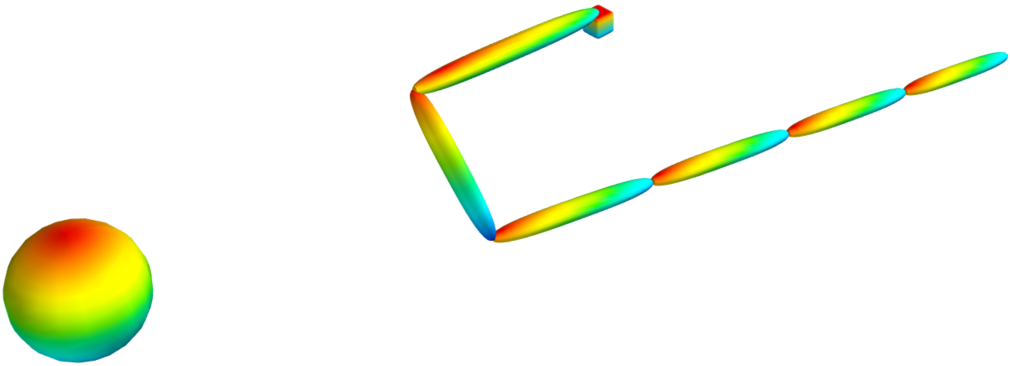
\includegraphics[width=1\textwidth]{import/RRT_6DOFSTART2}
		\label{fig:Res6DoFStart}
	\end{minipage}
	\begin{minipage}[h]{0.3\textwidth}
	\centering
	\subcaption{Goal.}
	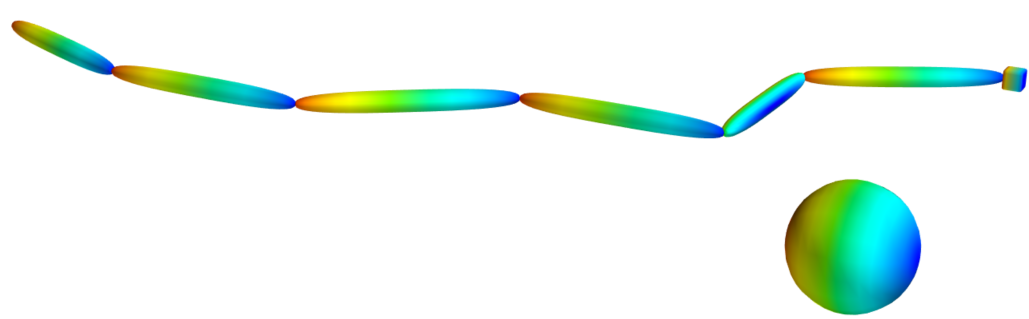
\includegraphics[width=1\textwidth]{import/RRT_6DOFGOAL2}
	\label{fig:Res6DoFGoal}
\end{minipage}

\end{figure}



\begin{figure}[h]
	\centering
	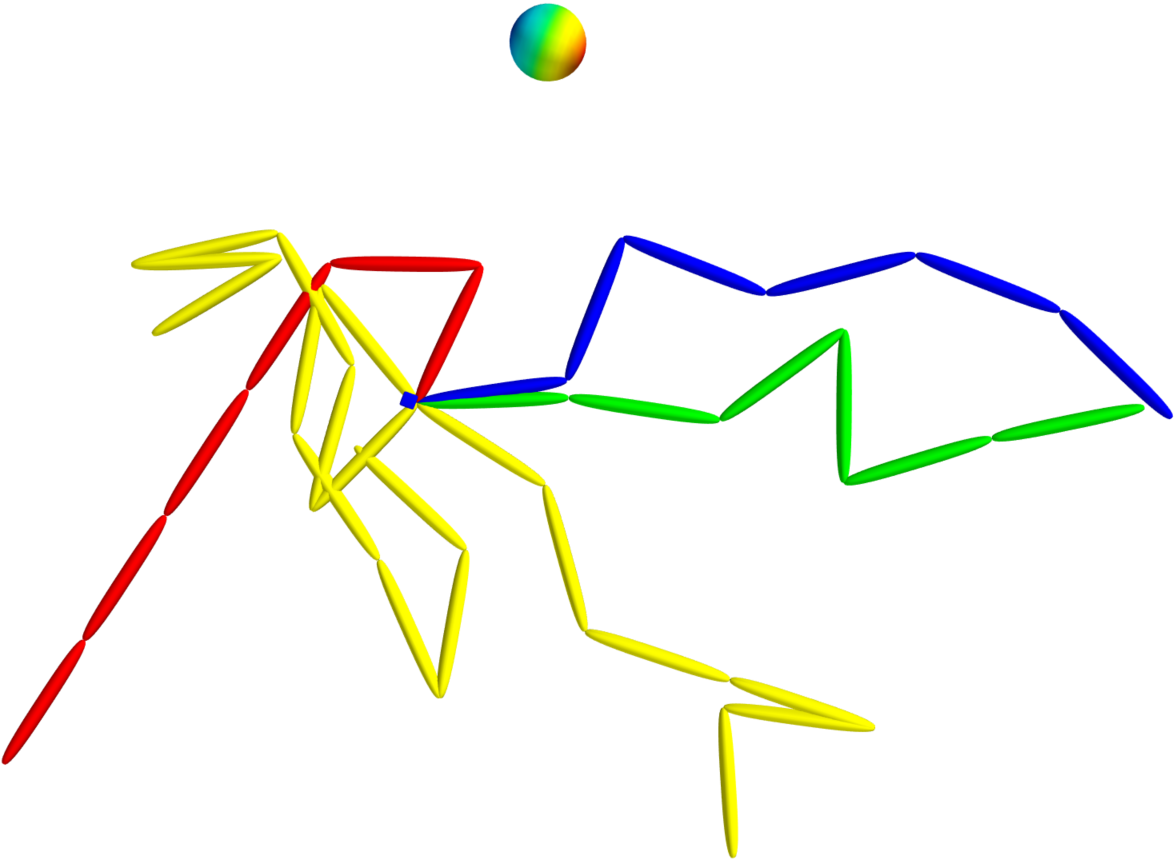
\includegraphics[width=0.5\textwidth]{import/RRT_6DOF_ex}
	\caption{Example of a motion plan, with various configurations over time. Red is the start configuration, blue is the provided goal configuration and green is the accepted returned final configuration. The yellow configurations are intermediary steps.}
	\label{fig:Res6DoFEx}
\end{figure}

Note that the algorithm returned \textit{a} motion plan in Figure \ref{fig:Res6DoFEx}, but not necessarily an optimal one by any measure.


%\begin{table}[h]
%	\begin{tabular}{|l|c|c|c|c|c|c|}
%		\hline
%		O\gls{SQ}				&	Test I		&	Test II		&	Test III	&	Test IV		&	Test V		&	Test VI	\\ \hline
%		Total Time {[}s{]}		&	8583		&	8308		&	1928		&	10954		&	3702		&	844		\\ \hline
%		Total loop iterations: 	&	28449		&	25346		&	6326		&	38059		&	15222		&	3909	\\ \hline
%		Collisions:				&	6245		&	6124		&	1672		&	10991		&	3758		&	1118	\\ \hline
%		Path node length:		&	7			&	7			&	6			&	6			&	7			&	6		\\ \hline
%	\end{tabular}
%	\caption{Result of the \gls{RRT} testing using O\gls{SQ}.}
%	\label{Table:RRTOSQ}
%\end{table}
%
%\begin{table}[h]
%	\begin{tabular}{|l|c|c|c|c|c|c|}
%		\hline
%		\gls{GJK}				&	Test I		&	Test II		&	Test III	&	Test IV		&	Test V		&	Test VI	\\ \hline
%		Total Time {[}s{]}		&	21812		&	6520		&	708			&	2648		&	148			&	2486	\\ \hline
%		Total loop iterations: 	&	14954		&	21525		&	2611		&	9623		&	521			&	8811	\\ \hline
%		Collisions:				&	3538		&	5244		&	771			&	3308		&	146			&	2073	\\ \hline
%		Path node length:		&	7			&	6			&	6			&	7			&	5			&	6		\\ \hline
%	\end{tabular}
%	\caption{Result of the \gls{RRT} testing using \gls{GJK}.}
%	\label{Table:RRTGJK}
%\end{table}
%
%
%\begin{table}[h]
%	\begin{tabular}{|l|c|c|c|c|c|c|}
%		\hline
%		R\gls{SQ}				&	Test I		&	Test II		&	Test III	&	Test IV		&	Test V		&	Test VI	\\ \hline
%		Total Time {[}s{]}		&	4150		&	5715		&	6506		&	780			&	5588		&	8109	\\ \hline
%		Total loop iterations: 	&	6193		&	20909		&	12284		&	3165		&	21128		&	31426	\\ \hline
%		Collisions:				&	1915		&	6874		&	4122		&	1062		&	5174		&	10670	\\ \hline
%		Path node length:		&	8			&	7			&		6		&		7		&		6		&	9		\\ \hline
%	\end{tabular}
%	\caption{Result of the \gls{RRT} testing using R\gls{SQ}.}
%	\label{Table:RRTRSQ}
%\end{table}



%OSQ:
%
%[22204, 20728, 19547, 13367, 3, 2, 0]
%('total count:', 28449)
%('RRT: ', 8583.148000001907)
%
%
%[[[0.0, 0.0, 0.0], [0.0, -4.8261607132300695, 0.0], [0.0, -8.168040405429899, 0.0], [0.0, -5.929810471951761, 0.0], [0.0, -4.986726658383635, 0.0], [0.0, -1.1044507749037529, 0.0], [0.0, -6.29572518501959, 0.0]], [[0.0, 0.0, 0.0], [0.0, -3.0146023112828715, 0.0], [0.0, -5.871608517680685, 0.0], [0.0, -4.054610749453104, 0.0], [0.0, -3.9242751265581237, 0.0], [0.0, -1.0946179255124986, 0.0], [0.0, -3.8138187793341993, 0.0]], [[0.0, 0.0, 0.0], [0.0, -1.4886627501391625, 0.0], [0.0, -3.654027810317971, 0.0], [0.0, -2.5457161870270397, 0.0], [0.0, -3.6047460441749744, 0.0], [0.0, -1.0819833697981434, 0.0], [0.0, -2.3033257559344245, 0.0]], [[0.0, 0.0, 0.0], [0.0, -0.9168274651045456, 0.0], [0.0, -1.9233980893317462, 0.0], [0.0, -1.5297695350831555, 0.0], [0.0, -3.4045053828083844, 0.0], [0.0, -1.0683125015093498, 0.0], [0.0, -1.6425873176518706, 0.0]], [[0.0, 0.0, 0.0], [0.0, -0.6917017196402695, 0.0], [0.0, -0.5445110247132586, 0.0], [0.0, -1.0139579451821414, 0.0], [0.0, -3.1523656695805506, 0.0], [0.0, -0.8657667230456635, 0.0], [0.0, -1.5281106196265415, 0.0]], [[0.0, 0.0, 0.0], [0.0, 1.41149818856956, 0.0], [0.0, -0.26099714999497525, 0.0], [0.0, 0.7724895032730376, 0.0], [0.0, -1.9557169790556415, 0.0], [0.0, -0.5051677932757728, 0.0], [0.0, -0.24297302377260033, 0.0]], [[0, 0, 0], [0, 1.5, 0], [0, 2, 0], [0, 1, 0], [0, 0, 0], [0, 0, 0], [0, 0, 0]]]
%
%
%[19222, 8577, 129, 7, 3, 2, 0]
%('total count:', 25346)
%('RRT: ', 8308.172999858856)
%[[[0.0, 0.0, 0.0], [0.0, -5.670896996108294, 0.0], [0.0, -1.1876247442894736, 0.0], [0.0, -5.500210269482635, 0.0], [0.0, -5.887558851435529, 0.0], [0.0, -5.449368571414492, 0.0], [0.0, -8.005752501663714, 0.0]], [[0.0, 0.0, 0.0], [0.0, -3.76191422560685, 0.0], [0.0, -1.0514383940386534, 0.0], [0.0, -3.9488642340318503, 0.0], [0.0, -3.9826975373846953, 0.0], [0.0, -3.7274109764422847, 0.0], [0.0, -5.413465268504888, 0.0]], [[0.0, 0.0, 0.0], [0.0, -2.4947283925374433, 0.0], [0.0, -0.9859197724803128, 0.0], [0.0, -2.5856716303880694, 0.0], [0.0, -2.8024576247639503, 0.0], [0.0, -2.688262432652394, 0.0], [0.0, -3.8169006070939973, 0.0]], [[0.0, 0.0, 0.0], [0.0, -1.0929526077091982, 0.0], [0.0, -0.013889577238222484, 0.0], [0.0, -1.5016855685865431, 0.0], [0.0, -1.885596853658134, 0.0], [0.0, -2.6873455884922732, 0.0], [0.0, -3.5783603008788996, 0.0]], [[0.0, 0.0, 0.0], [0.0, 0.5390435833269915, 0.0], [0.0, 0.3473595218593892, 0.0], [0.0, -0.9089088156985052, 0.0], [0.0, -1.5229238816241555, 0.0], [0.0, -2.3032852068867227, 0.0], [0.0, -2.4737896325943374, 0.0]], [[0.0, 0.0, 0.0], [0.0, 1.3856754643484237, 0.0], [0.0, 0.8319571965453405, 0.0], [0.0, 0.9528348606726913, 0.0], [0.0, -0.15112405463106762, 0.0], [0.0, -1.7175116953481124, 0.0], [0.0, -1.576539901650622, 0.0]], [[0, 0, 0], [0, 1.5, 0], [0, 2, 0], [0, 1, 0], [0, 0, 0], [0, 0, 0], [0, 0, 0]]]
%
%
%[4654, 28, 3, 2, 0]
%('total count:', 6326)
%('RRT: ', 1928.9559998512268)
%[[[0.0, 0.0, 0.0], [0.0, -5.180550967045235, 0.0], [0.0, -2.206890166842226, 0.0], [0.0, -4.62466098222416, 0.0], [0.0, -6.640517604171324, 0.0], [0.0, -5.635970527389518, 0.0], [0.0, -6.986651634494501, 0.0]], [[0.0, 0.0, 0.0], [0.0, -3.2275996486988747, 0.0], [0.0, -1.4647218840701677, 0.0], [0.0, -2.7894836724295926, 0.0], [0.0, -4.384896416286866, 0.0], [0.0, -3.709703405621199, 0.0], [0.0, -4.476525270606289, 0.0]], [[0.0, 0.0, 0.0], [0.0, -2.167119644509092, 0.0], [0.0, -0.5836731271881308, 0.0], [0.0, -2.5931790316035226, 0.0], [0.0, -3.594359485478721, 0.0], [0.0, -1.4739223443549936, 0.0], [0.0, -3.669742656835062, 0.0]], [[0.0, 0.0, 0.0], [0.0, -0.03947966600830877, 0.0], [0.0, 0.9015137646041367, 0.0], [0.0, -0.9923815632292889, 0.0], [0.0, -1.93251756733598, 0.0], [0.0, -0.41579802572637486, 0.0], [0.0, -1.4081529825416046, 0.0]], [[0, 0, 0], [0, 1.5, 0], [0, 2, 0], [0, 1, 0], [0, 0, 0], [0, 0, 0], [0, 0, 0]]]
%
%
%[27068, 358, 255, 9, 2, 0]
%('total count:', 38059)
%('RRT: ', 10954.126999855042)
%[[[0.0, 0.0, 0.0], [0.0, -6.958932368683811, 0.0], [0.0, -5.041628213415211, 0.0], [0.0, -6.69095245237455, 0.0], [0.0, -6.147573883718454, 0.0], [0.0, -6.418120336594956, 0.0], [0.0, -4.670156259487403, 0.0]], [[0.0, 0.0, 0.0], [0.0, -4.7615958592753564, 0.0], [0.0, -3.540763534247745, 0.0], [0.0, -4.326970985213757, 0.0], [0.0, -4.389207849443112, 0.0], [0.0, -4.300571526228406, 0.0], [0.0, -3.1514466162215062, 0.0]], [[0.0, 0.0, 0.0], [0.0, -2.787919072930527, 0.0], [0.0, -1.6034078303867423, 0.0], [0.0, -3.4045098579569686, 0.0], [0.0, -3.5966739542178208, 0.0], [0.0, -3.613635950283111, 0.0], [0.0, -2.826171928548674, 0.0]], [[0.0, 0.0, 0.0], [0.0, -1.3843714136339056, 0.0], [0.0, -0.3670254644001969, 0.0], [0.0, -2.316318148827243, 0.0], [0.0, -3.5222620826947195, 0.0], [0.0, -2.2317331266903353, 0.0], [0.0, -2.235946260251051, 0.0]], [[0.0, 0.0, 0.0], [0.0, -0.9941313597361381, 0.0], [0.0, 0.4845512397408558, 0.0], [0.0, -1.4067577297362321, 0.0], [0.0, -3.1204730443651307, 0.0], [0.0, -0.598099896389913, 0.0], [0.0, -0.14580510448677944, 0.0]], [[0, 0, 0], [0, 1.5, 0], [0, 2, 0], [0, 1, 0], [0, 0, 0], [0, 0, 0], [0, 0, 0]]]
%
%
%[11464, 7643, 6868, 2523, 82, 2, 0]
%('total count:', 15222)
%('RRT: ', 3702.901999950409)
%[[[0.0, 0.0, 0.0], [0.0, -5.903015053015704, 0.0], [0.0, -6.008659793325638, 0.0], [0.0, -6.022191109432825, 0.0], [0.0, -7.312885286255331, 0.0], [0.0, -6.886308380191317, 0.0], [0.0, -4.626994827377688, 0.0]], [[0.0, 0.0, 0.0], [0.0, -3.94761580562653, 0.0], [0.0, -3.974845336143292, 0.0], [0.0, -3.9837691447601173, 0.0], [0.0, -5.285306039115987, 0.0], [0.0, -4.549652634347608, 0.0], [0.0, -3.3036971519467766, 0.0]], [[0.0, 0.0, 0.0], [0.0, -2.1969897120178765, 0.0], [0.0, -2.0914923252855986, 0.0], [0.0, -2.5043411851735184, 0.0], [0.0, -3.275214751059207, 0.0], [0.0, -3.2714354211379466, 0.0], [0.0, -2.801279560273603, 0.0]], [[0.0, 0.0, 0.0], [0.0, -1.558267898230044, 0.0], [0.0, -1.1921763430619188, 0.0], [0.0, -1.8385999359427543, 0.0], [0.0, -2.0408710506889607, 0.0], [0.0, -2.4001186034061357, 0.0], [0.0, -2.7909762442767017, 0.0]], [[0.0, 0.0, 0.0], [0.0, -0.7243031464296118, 0.0], [0.0, -0.44593587431582027, 0.0], [0.0, -1.1046872394095546, 0.0], [0.0, -1.6191834992419327, 0.0], [0.0, -1.871965584771464, 0.0], [0.0, -2.7791642565538837, 0.0]], [[0.0, 0.0, 0.0], [0.0, -0.6450627224724883, 0.0], [0.0, 0.04736736779332018, 0.0], [0.0, 0.28936977540130726, 0.0], [0.0, -1.4809244329812925, 0.0], [0.0, -0.5782158571602453, 0.0], [0.0, -2.640236258985805, 0.0]], [[0, 0, 0], [0, 1.5, 0], [0, 2, 0], [0, 1, 0], [0, 0, 0], [0, 0, 0], [0, 0, 0]]]
%
%[2791, 619, 31, 3, 2, 1, 0]
%('total count:', 3909)
%('RRT: ', 844.0699999332428)
%[[[0.0, 0.0, 0.0], [0.0, -6.176320744780465, 0.0], [0.0, -5.363288187755952, 0.0], [0.0, -7.307366289301395, 0.0], [0.0, -6.23936398393185, 0.0], [0.0, -4.836276597188812, 0.0], [0.0, -2.074128451269762, 0.0]], [[0.0, 0.0, 0.0], [0.0, -4.018951705849035, 0.0], [0.0, -3.3671040947634223, 0.0], [0.0, -4.459021215526185, 0.0], [0.0, -3.937543903398658, 0.0], [0.0, -3.020643904031561, 0.0], [0.0, -1.6008732173875577, 0.0]], [[0.0, 0.0, 0.0], [0.0, -3.0957183884669446, 0.0], [0.0, -2.469625167728175, 0.0], [0.0, -3.012059585998401, 0.0], [0.0, -2.3511928341052304, 0.0], [0.0, -1.7698031497482123, 0.0], [0.0, -1.4848827676710885, 0.0]], [[0.0, 0.0, 0.0], [0.0, -2.6302363465245158, 0.0], [0.0, -0.7109245038983185, 0.0], [0.0, -2.781057357402486, 0.0], [0.0, -2.024787659476211, 0.0], [0.0, -1.1780817671687194, 0.0], [0.0, -1.1118189054587542, 0.0]], [[0.0, 0.0, 0.0], [0.0, 0.14475975395210905, 0.0], [0.0, 1.566223586852641, 0.0], [0.0, -1.7074974219609698, 0.0], [0.0, -0.19143188360248165, 0.0], [0.0, -0.9239674154596824, 0.0], [0.0, -0.4799596022252783, 0.0]], [[0.0, 0.0, 0.0], [0.0, 1.7617993877991494, 0.0], [0.0, 2.5235987755982987, 0.0], [0.0, 0.21460183660255172, 0.0], [0.0, 0.3141592653589793, 0.0], [0.0, -0.3141592653589793, 0.0], [0.0, -0.19634954084936207, 0.0]], [[0, 0, 0], [0, 1.5, 0], [0, 2, 0], [0, 1, 0], [0, 0, 0], [0, 0, 0], [0, 0, 0]]]


%GJK:
%
%[11416, 5970, 5504, 5049, 10, 2, 0]
%('total count:', 14954)
%('RRT: ', 21811.72199988365)
%[[[0.0, 0.0, 0.0], [0.0, -6.876071730600213, 0.0], [0.0, -5.949965930081643, 0.0], [0.0, -5.820817405275493, 0.0], [0.0, -4.93363386331143, 0.0], [0.0, -7.0178566462387755, 0.0], [0.0, -6.597371481480376, 0.0]], [[0.0, 0.0, 0.0], [0.0, -4.290957316716859, 0.0], [0.0, -3.78919121531564, 0.0], [0.0, -4.070886030265919, 0.0], [0.0, -3.5861934016032837, 0.0], [0.0, -4.75662721680071, 0.0], [0.0, -4.565305801983427, 0.0]], [[0.0, 0.0, 0.0], [0.0, -2.61726968042678, 0.0], [0.0, -2.4929676915823853, 0.0], [0.0, -2.503028822647307, 0.0], [0.0, -2.8480418760692645, 0.0], [0.0, -3.042811061763742, 0.0], [0.0, -3.4614047341038905, 0.0]], [[0.0, 0.0, 0.0], [0.0, -1.822661703875945, 0.0], [0.0, -1.5761638123639519, 0.0], [0.0, -1.4899983200673916, 0.0], [0.0, -2.5735583517971716, 0.0], [0.0, -1.8667543343220179, 0.0], [0.0, -2.8333384286568393, 0.0]], [[0.0, 0.0, 0.0], [0.0, -0.7558135581591037, 0.0], [0.0, -1.4606881243666248, 0.0], [0.0, -0.27590224485511394, 0.0], [0.0, -2.446266116366309, 0.0], [0.0, -1.5091464086695772, 0.0], [0.0, -2.275486780994961, 0.0]], [[0.0, 0.0, 0.0], [0.0, 0.03046120467588942, 0.0], [0.0, -0.9457966959175295, 0.0], [0.0, 0.6776416928814748, 0.0], [0.0, -2.3260697852292957, 0.0], [0.0, -1.4915789766696297, 0.0], [0.0, -1.1020060779462202, 0.0]], [[0, 0, 0], [0, 1.5, 0], [0, 2, 0], [0, 1, 0], [0, 0, 0], [0, 0, 0], [0, 0, 0]]]
%
%[16281, 2459, 731, 408, 2, 0]
%('total count:', 21525)
%('RRT: ', 6519.712999820709)
%[[[0.0, 0.0, 0.0], [0.0, -0.4150177791342668, 0.0], [0.0, -5.968281106269311, 0.0], [0.0, -5.467045500083865, 0.0], [0.0, -6.404408592816946, 0.0], [0.0, -5.494024220411203, 0.0], [0.0, -7.480796578936015, 0.0]], [[0.0, 0.0, 0.0], [0.0, -0.2560686778224509, 0.0], [0.0, -3.857389846886636, 0.0], [0.0, -3.4748074891546272, 0.0], [0.0, -4.155455300371088, 0.0], [0.0, -3.564673333397604, 0.0], [0.0, -4.872823041383114, 0.0]], [[0.0, 0.0, 0.0], [0.0, -0.1247338561428959, 0.0], [0.0, -2.5995371959857363, 0.0], [0.0, -1.9935705892992535, 0.0], [0.0, -2.462853923682264, 0.0], [0.0, -2.3644127140061606, 0.0], [0.0, -3.0798130639153958, 0.0]], [[0.0, 0.0, 0.0], [0.0, -0.10723662940797973, 0.0], [0.0, -1.7271190176870255, 0.0], [0.0, -1.184084106744792, 0.0], [0.0, -1.0762485493853515, 0.0], [0.0, -1.9279198210055277, 0.0], [0.0, -2.941203317633166, 0.0]], [[0.0, 0.0, 0.0], [0.0, 0.3788878941248819, 0.0], [0.0, -0.867532501418399, 0.0], [0.0, -0.302320446317371, 0.0], [0.0, -0.2741710254259186, 0.0], [0.0, -1.9031428133842268, 0.0], [0.0, -2.557826086270656, 0.0]], [[0, 0, 0], [0, 1.5, 0], [0, 2, 0], [0, 1, 0], [0, 0, 0], [0, 0, 0], [0, 0, 0]]]
%
%
%[1840, 463, 3, 2, 1, 0]
%('total count:', 2611)
%('RRT: ', 708.3889999389648)
%[[[0.0, 0.0, 0.0], [0.0, -5.686665798690559, 0.0], [0.0, -6.545621976826601, 0.0], [0.0, -7.553647998662415, 0.0], [0.0, -4.947675435300449, 0.0], [0.0, -5.990191950430879, 0.0], [0.0, -6.183322155887421, 0.0]], [[0.0, 0.0, 0.0], [0.0, -3.3603675231318997, 0.0], [0.0, -4.1083168298203585, 0.0], [0.0, -5.252020902153491, 0.0], [0.0, -3.409616069659995, 0.0], [0.0, -4.071967687499828, 0.0], [0.0, -4.13244481218558, 0.0]], [[0.0, 0.0, 0.0], [0.0, -1.5917783397147143, 0.0], [0.0, -2.480615701446832, 0.0], [0.0, -3.359321726637443, 0.0], [0.0, -1.6689514545830675, 0.0], [0.0, -3.5757226572492815, 0.0], [0.0, -3.2230250236314912, 0.0]], [[0.0, 0.0, 0.0], [0.0, -0.6879073799798248, 0.0], [0.0, 0.23199385061844024, 0.0], [0.0, -2.06544628664295, 0.0], [0.0, -0.2112426319084122, 0.0], [0.0, -3.2756199699833037, 0.0], [0.0, -1.996729936503588, 0.0]], [[0.0, 0.0, 0.0], [0.0, 1.7617993877991494, 0.0], [0.0, 2.5235987755982987, 0.0], [0.0, 0.21460183660255172, 0.0], [0.0, 0.3141592653589793, 0.0], [0.0, -0.3141592653589793, 0.0], [0.0, -0.19634954084936207, 0.0]], [[0, 0, 0], [0, 1.5, 0], [0, 2, 0], [0, 1, 0], [0, 0, 0], [0, 0, 0], [0, 0, 0]]]
%
%[6315, 2814, 2667, 1811, 2, 1, 0]
%('total count:', 9623)
%('RRT: ', 2648.225000143051)
%[[[0.0, 0.0, 0.0], [0.0, -5.074076619598711, 0.0], [0.0, -0.17631605315247245, 0.0], [0.0, -7.8809960258506075, 0.0], [0.0, -5.261897533054691, 0.0], [0.0, -7.273599976961859, 0.0], [0.0, -5.357217945446061, 0.0]], [[0.0, 0.0, 0.0], [0.0, -3.2395744292820385, 0.0], [0.0, -0.10527953068998272, 0.0], [0.0, -5.081602603283653, 0.0], [0.0, -3.7085888965779343, 0.0], [0.0, -5.327069737589381, 0.0], [0.0, -3.441014238060995, 0.0]], [[0.0, 0.0, 0.0], [0.0, -2.3197129716881455, 0.0], [0.0, -0.05012444222056445, 0.0], [0.0, -3.610528281991487, 0.0], [0.0, -2.496492292190638, 0.0], [0.0, -3.2343393874064503, 0.0], [0.0, -2.1151311843111107, 0.0]], [[0.0, 0.0, 0.0], [0.0, -1.2280575885123652, 0.0], [0.0, 0.34889884385515635, 0.0], [0.0, -3.556827871685475, 0.0], [0.0, -1.2180076342309052, 0.0], [0.0, -2.7819581751640423, 0.0], [0.0, -1.6746180451188342, 0.0]], [[0.0, 0.0, 0.0], [0.0, 0.14921696405502782, 0.0], [0.0, 0.5810592451390881, 0.0], [0.0, -2.812905228306603, 0.0], [0.0, -0.7650633664542501, 0.0], [0.0, -2.6512141940690253, 0.0], [0.0, -1.4295873599807016, 0.0]], [[0.0, 0.0, 0.0], [0.0, 1.7617993877991494, 0.0], [0.0, 2.5235987755982987, 0.0], [0.0, 0.21460183660255172, 0.0], [0.0, 0.3141592653589793, 0.0], [0.0, -0.3141592653589793, 0.0], [0.0, -0.19634954084936207, 0.0]], [[0, 0, 0], [0, 1.5, 0], [0, 2, 0], [0, 1, 0], [0, 0, 0], [0, 0, 0], [0, 0, 0]]]
%
%
%[375, 158, 19, 2, 0]
%('total count:', 521)
%('RRT: ', 147.84400010108948)
%[[[0.0, 0.0, 0.0], [0.0, -5.873676971345004, 0.0], [0.0, -6.464538978006821, 0.0], [0.0, 0.7780870516557586, 0.0], [0.0, -8.488061726768128, 0.0], [0.0, -4.41379123617278, 0.0], [0.0, -6.373785014552839, 0.0]], [[0.0, 0.0, 0.0], [0.0, -3.6575935200544123, 0.0], [0.0, -4.009221523104698, 0.0], [0.0, 0.7787620538159293, 0.0], [0.0, -6.459969495396895, 0.0], [0.0, -3.733412447554529, 0.0], [0.0, -4.538010108805495, 0.0]], [[0.0, 0.0, 0.0], [0.0, -1.9727508813851968, 0.0], [0.0, -2.6484132179466435, 0.0], [0.0, 0.7945117995006243, 0.0], [0.0, -5.012267874872514, 0.0], [0.0, -3.30521460114529, 0.0], [0.0, -2.6585535987026496, 0.0]], [[0.0, 0.0, 0.0], [0.0, -0.19370555968406888, 0.0], [0.0, -0.7376546015950458, 0.0], [0.0, 0.9888480918450452, 0.0], [0.0, -3.034662945196151, 0.0], [0.0, -2.954372838484962, 0.0], [0.0, -1.7649372531644578, 0.0]], [[0, 0, 0], [0, 1.5, 0], [0, 2, 0], [0, 1, 0], [0, 0, 0], [0, 0, 0], [0, 0, 0]]]
%
%
%[6738, 315, 89, 6, 2, 0]
%('total count:', 8811)
%('RRT: ', 2486.140000104904)
%[[[0.0, 0.0, 0.0], [0.0, -5.438859428765257, 0.0], [0.0, -7.54384863086337, 0.0], [0.0, -4.301301223637902, 0.0], [0.0, -7.277624662505487, 0.0], [0.0, -7.123535334716889, 0.0], [0.0, -5.819750886926878, 0.0]], [[0.0, 0.0, 0.0], [0.0, -3.7230289261517093, 0.0], [0.0, -5.236597671705908, 0.0], [0.0, -2.915995813537633, 0.0], [0.0, -5.052908797140172, 0.0], [0.0, -4.913115774115894, 0.0], [0.0, -3.8135373306020934, 0.0]], [[0.0, 0.0, 0.0], [0.0, -2.287306707403076, 0.0], [0.0, -3.9645847997657873, 0.0], [0.0, -2.11196567623005, 0.0], [0.0, -3.7048558412094494, 0.0], [0.0, -3.2824585780138533, 0.0], [0.0, -2.798322758821795, 0.0]], [[0.0, 0.0, 0.0], [0.0, -1.3462827286525854, 0.0], [0.0, -2.519218523838927, 0.0], [0.0, -1.6754032234518823, 0.0], [0.0, -3.4801756311231786, 0.0], [0.0, -1.717442200276997, 0.0], [0.0, -2.14007183054804, 0.0]], [[0.0, 0.0, 0.0], [0.0, -0.7022854631374478, 0.0], [0.0, 0.5272239413433293, 0.0], [0.0, -0.9789968107944551, 0.0], [0.0, -1.9527244160177006, 0.0], [0.0, -1.4729379357624943, 0.0], [0.0, -0.8051267604519454, 0.0]], [[0, 0, 0], [0, 1.5, 0], [0, 2, 0], [0, 1, 0], [0, 0, 0], [0, 0, 0], [0, 0, 0]]]




%RSQ:
%
%[4278, 2340, 1093, 157, 140, 48, 1, 0]
%('total count:', 6193)
%('RRT: ', 4149.572000026703)
%[[[0.0, 0.0, 0.0], [0.0, -6.235094718192088, 0.0], [0.0, -6.388870508717041, 0.0], [0.0, -4.33897821929162, 0.0], [0.0, -1.7407640221725758, 0.0], [0.0, -6.156267968175465, 0.0], [0.0, -6.02394653806201, 0.0]], [[0.0, 0.0, 0.0], [0.0, -4.2520670112236605, 0.0], [0.0, -3.4441764420001393, 0.0], [0.0, -4.209112570134844, 0.0], [0.0, -1.4641605386354177, 0.0], [0.0, -4.361492559610188, 0.0], [0.0, -3.531655721370509, 0.0]], [[0.0, 0.0, 0.0], [0.0, -3.033854388204408, 0.0], [0.0, -1.487122947629774, 0.0], [0.0, -4.036286317955362, 0.0], [0.0, -0.9178482118203886, 0.0], [0.0, -3.985112748705846, 0.0], [0.0, -2.389308997375408, 0.0]], [[0.0, 0.0, 0.0], [0.0, -2.3207037465601257, 0.0], [0.0, -0.25134455787357446, 0.0], [0.0, -3.7370421576096193, 0.0], [0.0, -0.7058209241039033, 0.0], [0.0, -3.5666814885986047, 0.0], [0.0, -1.1723464915203348, 0.0]], [[0.0, 0.0, 0.0], [0.0, -0.6487113662423833, 0.0], [0.0, 1.5260445500033952, 0.0], [0.0, -3.0937963089006595, 0.0], [0.0, -0.2104466864342938, 0.0], [0.0, -2.400481239616072, 0.0], [0.0, -0.8326171993483085, 0.0]], [[0.0, 0.0, 0.0], [0.0, 0.3582115333036162, 0.0], [0.0, 2.177132322573485, 0.0], [0.0, -2.671182678977206, 0.0], [0.0, 0.10468673719020768, 0.0], [0.0, -1.4886933313678594, 0.0], [0.0, -0.3320134880222173, 0.0]], [[0.0, 0.0, 0.0], [0.0, 1.7617993877991494, 0.0], [0.0, 2.5235987755982987, 0.0], [0.0, 0.21460183660255172, 0.0], [0.0, 0.3141592653589793, 0.0], [0.0, -0.3141592653589793, 0.0], [0.0, -0.19634954084936207, 0.0]], [[0, 0, 0], [0, 1.5, 0], [0, 2, 0], [0, 1, 0], [0, 0, 0], [0, 0, 0], [0, 0, 0]]]
%
%
%
%
%
%[14035, 9595, 5641, 3331, 114, 2, 0]
%('total count:', 20909)
%('RRT: ', 5715.125)
%[[[0.0, 0.0, 0.0], [0.0, -5.273072089435638, 0.0], [0.0, -1.0795770562766476, 0.0], [0.0, -6.788764296986185, 0.0], [0.0, -5.972463422249586, 0.0], [0.0, -5.0862318712408365, 0.0], [0.0, -6.3994043250754045, 0.0]], [[0.0, 0.0, 0.0], [0.0, -3.1619414267373607, 0.0], [0.0, -1.0609171246142355, 0.0], [0.0, -4.4166157928939676, 0.0], [0.0, -4.0687411174409895, 0.0], [0.0, -3.1599652756635845, 0.0], [0.0, -4.075685604073605, 0.0]], [[0.0, 0.0, 0.0], [0.0, -1.987455944778683, 0.0], [0.0, -0.8370788335172297, 0.0], [0.0, -2.437820404719327, 0.0], [0.0, -3.333569449175335, 0.0], [0.0, -2.601928526096205, 0.0], [0.0, -2.406932671760064, 0.0]], [[0.0, 0.0, 0.0], [0.0, -1.5160891788435857, 0.0], [0.0, -0.5127823126291196, 0.0], [0.0, -1.5098632881639613, 0.0], [0.0, -3.1802573573078488, 0.0], [0.0, -2.4463964306629578, 0.0], [0.0, -1.3858988113969586, 0.0]], [[0.0, 0.0, 0.0], [0.0, -1.1071763240588466, 0.0], [0.0, -0.01651290747484191, 0.0], [0.0, -0.343788053886923, 0.0], [0.0, -3.1384595194137916, 0.0], [0.0, -2.0119608640787394, 0.0], [0.0, -1.0178944286573754, 0.0]], [[0.0, 0.0, 0.0], [0.0, -0.47230181093203405, 0.0], [0.0, 0.6705681850435732, 0.0], [0.0, 0.34159195020096667, 0.0], [0.0, -2.9702910491937375, 0.0], [0.0, -0.6576001744623985, 0.0], [0.0, -0.9207805862392595, 0.0]], [[0, 0, 0], [0, 1.5, 0], [0, 2, 0], [0, 1, 0], [0, 0, 0], [0, 0, 0], [0, 0, 0]]]
%
%
%[8162, 914, 335, 9, 2, 0]
%('total count:', 12284)
%('RRT: ', 6505.578000068665)
%[[[0.0, 0.0, 0.0], [0.0, -5.422665360558103, 0.0], [0.0, -6.487431886528295, 0.0], [0.0, -0.975883501585413, 0.0], [0.0, -6.06109550506186, 0.0], [0.0, -4.718419040620013, 0.0], [0.0, -8.25641608378146, 0.0]], [[0.0, 0.0, 0.0], [0.0, -3.375063240672763, 0.0], [0.0, -4.227660364200356, 0.0], [0.0, -0.42452532492740525, 0.0], [0.0, -4.3258940323560395, 0.0], [0.0, -3.0548777645943375, 0.0], [0.0, -5.587113050057399, 0.0]], [[0.0, 0.0, 0.0], [0.0, -1.966600582960539, 0.0], [0.0, -2.5556677416072633, 0.0], [0.0, -0.16172860533697622, 0.0], [0.0, -3.1832162554892385, 0.0], [0.0, -2.1822655220351863, 0.0], [0.0, -3.6398767424912606, 0.0]], [[0.0, 0.0, 0.0], [0.0, -1.8023265855310924, 0.0], [0.0, -1.216656144103317, 0.0], [0.0, 0.013468165276277533, 0.0], [0.0, -1.462195857549588, 0.0], [0.0, -2.118363125973201, 0.0], [0.0, -2.52247257611345, 0.0]], [[0.0, 0.0, 0.0], [0.0, -1.1500441642652453, 0.0], [0.0, 0.6292229713986892, 0.0], [0.0, 0.19006067916620262, 0.0], [0.0, -0.553071910774724, 0.0], [0.0, -1.1879549299607914, 0.0], [0.0, -1.8404017887927624, 0.0]], [[0, 0, 0], [0, 1.5, 0], [0, 2, 0], [0, 1, 0], [0, 0, 0], [0, 0, 0], [0, 0, 0]]]
%
%
%
%[2103, 1147, 998, 29, 2, 1, 0]
%('total count:', 3165)
%('RRT: ', 779.8129999637604)
%[[[0.0, 0.0, 0.0], [0.0, -6.901587665479349, 0.0], [0.0, -4.639936907841659, 0.0], [0.0, -5.966244398437258, 0.0], [0.0, -7.834619411489333, 0.0], [0.0, -5.985428620304344, 0.0], [0.0, -5.8114355790113565, 0.0]], [[0.0, 0.0, 0.0], [0.0, -4.53367221762053, 0.0], [0.0, -3.4190706221955045, 0.0], [0.0, -3.9430415921649145, 0.0], [0.0, -4.812887475181481, 0.0], [0.0, -4.27643706842911, 0.0], [0.0, -3.9104535173139037, 0.0]], [[0.0, 0.0, 0.0], [0.0, -2.563711886164575, 0.0], [0.0, -2.223924375529064, 0.0], [0.0, -2.3019388247465473, 0.0], [0.0, -3.119198871833974, 0.0], [0.0, -3.839371894518555, 0.0], [0.0, -3.9031515056623105, 0.0]], [[0.0, 0.0, 0.0], [0.0, -1.7523989015113057, 0.0], [0.0, -1.2372941363918446, 0.0], [0.0, -1.7654049976271513, 0.0], [0.0, -1.5838062564996416, 0.0], [0.0, -3.607238169732821, 0.0], [0.0, -3.7081961200738407, 0.0]], [[0.0, 0.0, 0.0], [0.0, -0.7205496452353113, 0.0], [0.0, 0.7989729271146866, 0.0], [0.0, -1.7252953180984374, 0.0], [0.0, -0.7378811636531464, 0.0], [0.0, -3.160864024322317, 0.0], [0.0, -3.257782514422259, 0.0]], [[0.0, 0.0, 0.0], [0.0, 1.7617993877991494, 0.0], [0.0, 2.5235987755982987, 0.0], [0.0, 0.21460183660255172, 0.0], [0.0, 0.3141592653589793, 0.0], [0.0, -0.3141592653589793, 0.0], [0.0, -0.19634954084936207, 0.0]], [[0, 0, 0], [0, 1.5, 0], [0, 2, 0], [0, 1, 0], [0, 0, 0], [0, 0, 0], [0, 0, 0]]]
%
%
%
%
%
%
%[15954, 6933, 408, 393, 2, 0]
%('total count:', 21128)
%('RRT: ', 5587.52799987793)
%[[[0.0, 0.0, 0.0], [0.0, -4.628866251264537, 0.0], [0.0, -1.3676476398053148, 0.0], [0.0, -6.423547914957636, 0.0], [0.0, -5.854874579984349, 0.0], [0.0, -7.122087514002095, 0.0], [0.0, -6.097750716834775, 0.0]], [[0.0, 0.0, 0.0], [0.0, -2.7682993044843904, 0.0], [0.0, -1.2465255561607091, 0.0], [0.0, -4.21043263696928, 0.0], [0.0, -3.4771133650490107, 0.0], [0.0, -4.540731284298338, 0.0], [0.0, -4.090030597011531, 0.0]], [[0.0, 0.0, 0.0], [0.0, -1.9002297597623783, 0.0], [0.0, -1.2383908194061537, 0.0], [0.0, -2.828669253414184, 0.0], [0.0, -2.0513208033633443, 0.0], [0.0, -2.742563859466237, 0.0], [0.0, -3.6135187798900206, 0.0]], [[0.0, 0.0, 0.0], [0.0, -0.19754329750405752, 0.0], [0.0, -1.0762796367125662, 0.0], [0.0, -0.5717947745057627, 0.0], [0.0, -1.7271686910472257, 0.0], [0.0, -2.570829014853062, 0.0], [0.0, -3.2598443528726104, 0.0]], [[0.0, 0.0, 0.0], [0.0, 0.3510007581104524, 0.0], [0.0, -0.8116299585237079, 0.0], [0.0, 0.050974077414647434, 0.0], [0.0, -0.920526713990757, 0.0], [0.0, -2.5242114741444874, 0.0], [0.0, -2.8384819128946193, 0.0]], [[0, 0, 0], [0, 1.5, 0], [0, 2, 0], [0, 1, 0], [0, 0, 0], [0, 0, 0], [0, 0, 0]]]
%
%
%
%[20756, 13679, 4783, 1351, 1241, 1235, 1227, 571, 0]
%('total count:', 31426)
%('RRT: ', 8108.634999990463)
%[[[0.0, 0.0, 0.0], [0.0, -6.513918925911856, 0.0], [0.0, -5.212305766609874, 0.0], [0.0, -5.770634618452176, 0.0], [0.0, -7.9474258293582105, 0.0], [0.0, -5.50561764682037, 0.0], [0.0, -6.812775282395775, 0.0]], [[0.0, 0.0, 0.0], [0.0, -4.111800965847756, 0.0], [0.0, -3.7842422450327744, 0.0], [0.0, -3.897770675250653, 0.0], [0.0, -5.6000832489829335, 0.0], [0.0, -3.876042288470315, 0.0], [0.0, -4.6119321766125445, 0.0]], [[0.0, 0.0, 0.0], [0.0, -2.9172324488370833, 0.0], [0.0, -2.989399784911612, 0.0], [0.0, -2.551438931642773, 0.0], [0.0, -4.076748493412275, 0.0], [0.0, -2.3706553411655023, 0.0], [0.0, -3.101945522405998, 0.0]], [[0.0, 0.0, 0.0], [0.0, -2.218385698947066, 0.0], [0.0, -2.339109195099669, 0.0], [0.0, -1.6360673199023597, 0.0], [0.0, -3.379443153946819, 0.0], [0.0, -1.8985207866584033, 0.0], [0.0, -2.0870689186902953, 0.0]], [[0.0, 0.0, 0.0], [0.0, -1.6288950551292922, 0.0], [0.0, 0.28088452414739384, 0.0], [0.0, -0.38050773293425705, 0.0], [0.0, -3.0702894559456633, 0.0], [0.0, -1.5228280532408536, 0.0], [0.0, -1.3727657790145373, 0.0]], [[0.0, 0.0, 0.0], [0.0, -1.2277706923800573, 0.0], [0.0, 1.1301201584180363, 0.0], [0.0, 0.4258064089321553, 0.0], [0.0, -1.8468026815492238, 0.0], [0.0, -1.1830593655292618, 0.0], [0.0, -0.8292388152353701, 0.0]], [[0.0, 0.0, 0.0], [0.0, 0.030688599165887065, 0.0], [0.0, 1.653358915184249, 0.0], [0.0, 0.6170927123294974, 0.0], [0.0, -0.9000111113787688, 0.0], [0.0, -0.4517080381794641, 0.0], [0.0, -0.7971144719357444, 0.0]], [[0.0, 0.0, 0.0], [0.0, 0.7362911026909819, 0.0], [0.0, 1.9083309913533673, 0.0], [0.0, 0.7695292195953283, 0.0], [0.0, -0.3296553057577309, 0.0], [0.0, -0.1700870777101084, 0.0], [0.0, -0.5681227466023023, 0.0]], [[0, 0, 0], [0, 1.5, 0], [0, 2, 0], [0, 1, 0], [0, 0, 0], [0, 0, 0], [0, 0, 0]]]



